\chapter{Results}
\label{chapter:Results}

The final output of this work is twofold
\begin{itemize}
    \item{an evaluation of support vector machines and ensemble learning methods in the domain of text classification}
    \item{a web based interface that implements the evaluated techniques and presents a system which can monitor the public feed from the Internet to find out people who are suffering emotional distress and may need help}
\end{itemize}

\section{Evaluation}
\label{section:evaluation}
The evaluation of all algorithms used is done on the comments dataset \cite{kaggle}. To report online learning scores, the learning continues in iterations. In each iteration, 100 random samples are picked on which the models are trained and the accuracy is measured. This is continued until no more samples are left. All accuracies reported henceforth are calculated using hold-out cross-validation, training the model on 70\% of the data and testing on the remaining 30\%.

\subsection{SVM}
The behavior of SVM based classification depends heavily on the kernel being used. Using a linear kernel yields a cross validation accuracy of 79.06\%, while using either of polynomial/RBF/sigmoid kernels gives an accuracy of only 34.39\%. This can be attributed to the intuitive notion of how kernel functions operate. A kernel function calculates the similarity between vectors when the vectors have been transformed from their original low dimensional space into a high dimensional space. In the current scenario, the text corpus contains 23175 features, which is already a very high number. Any transformation from this space into an even higher space results in a decrease in the final accuracy calculated, as can be noted in the results.

\subsubsection{Accuracy}
When using a linear kernel, the accuracy of an SVM shows an increase as the number of input instances increases. The score ranges from 70.00\% when measuring on 100 samples, to 79.71\% when measuring on all 6182 samples, as shown in Figure~\ref{svm_accuracy}.
\begin{figure}
    \centering
    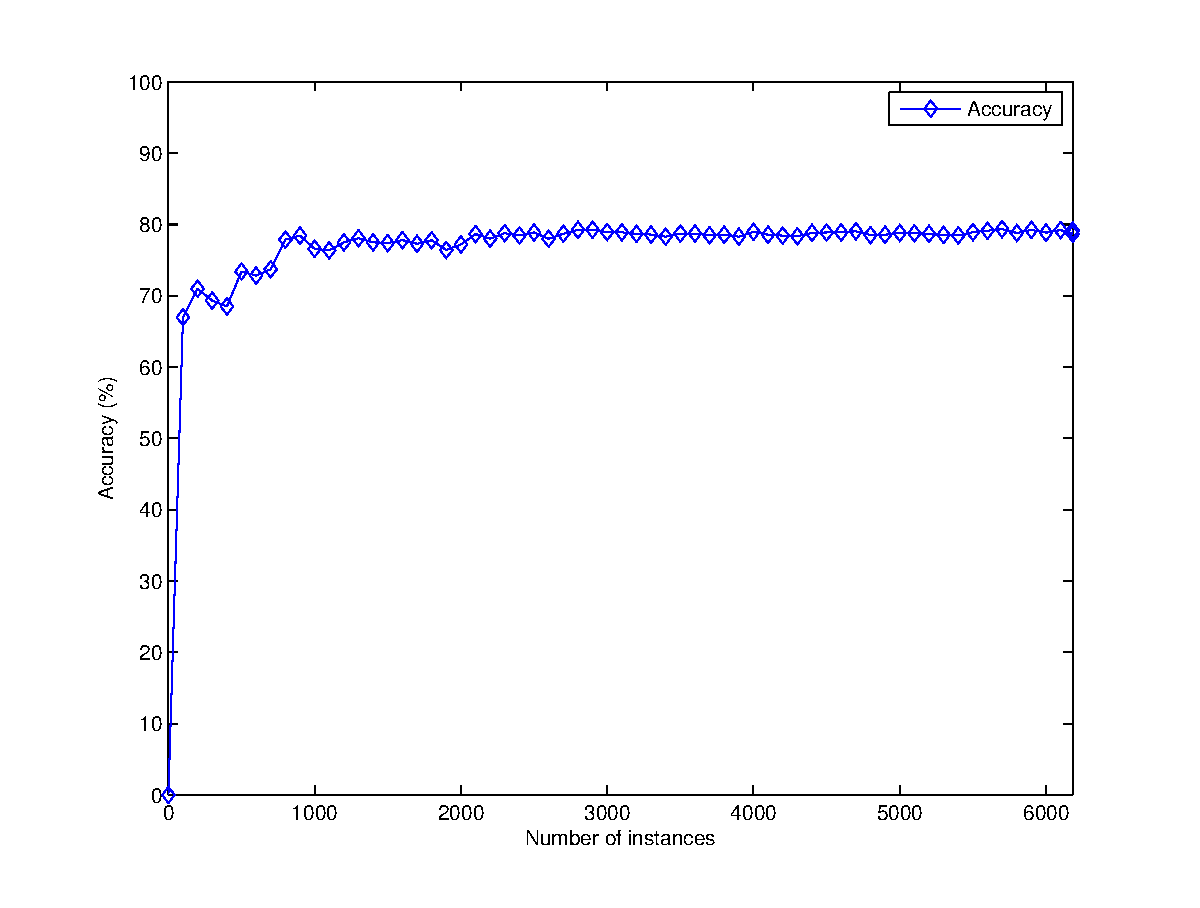
\includegraphics[scale=0.5]{svm_accuracy.eps}
    \caption{Accuracy of a linear kernel measured against the number of instances}
    \label{svm_accuracy}
\end{figure}

\subsubsection{Number of support vectors}
Support vectors is the subset of data points that the main classifier uses to establish the margin between the two class of points. Measuring the number of support vectors against the total number of instances gives an idea about the performance of the classifier - the more the number of support vectors (relative to the number of instances), the harder it is to perform a classification. Figure~\ref{svm_n_sv} shows this variation for the problem at hand. The number ranges from 70 for 100 samples to 3113 for 6182 samples, the increase being almost linear in the number of instances. It can be noted that the percentage decreases from 70\% to around 50\%, which shows that the more the information available to the classifier, the easier the task at hand becomes.
\begin{figure}
    \centering
    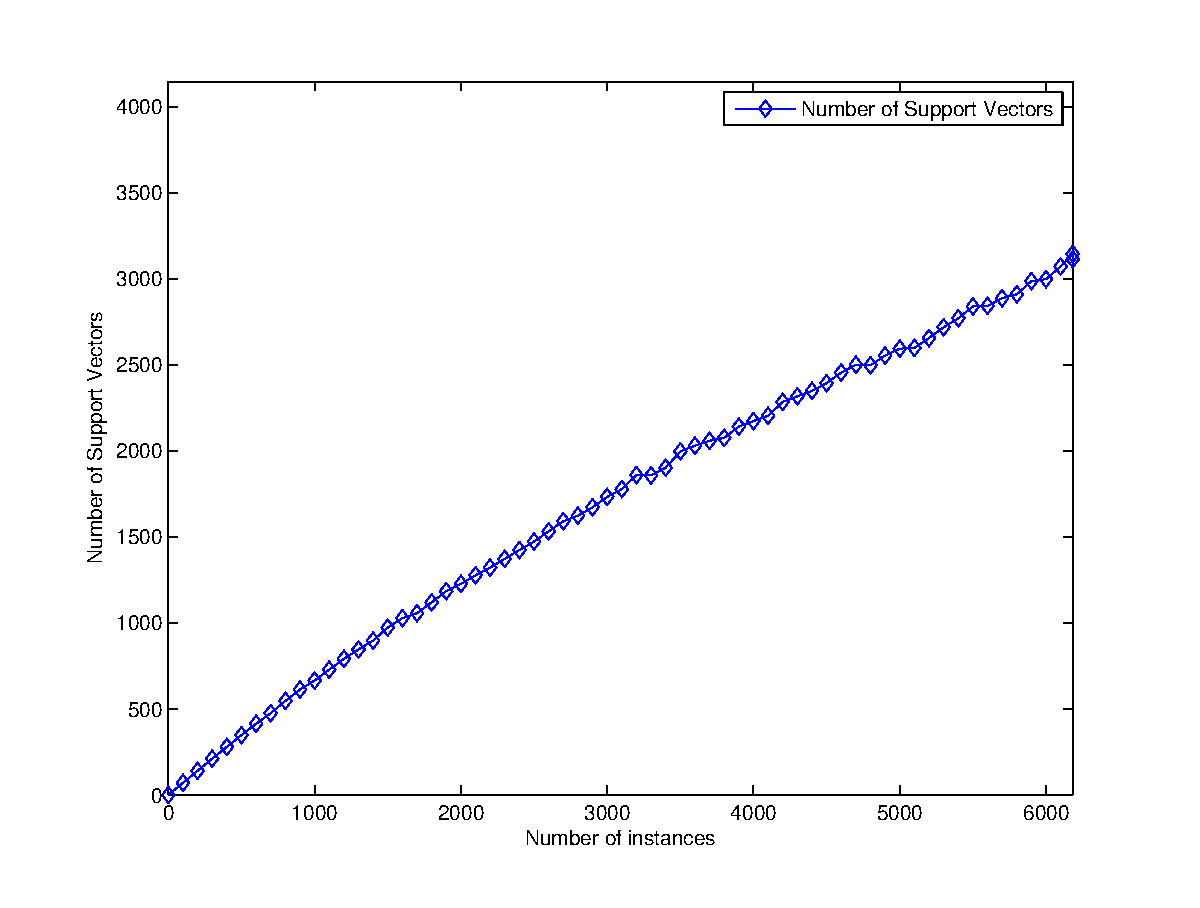
\includegraphics[scale=0.5]{svm_n_sv.eps}
    \caption{Variation of the number of support vectors in a linear kernel SVM, measured against the number of instances}
    \label{svm_n_sv}
\end{figure}

\subsection{Ensemble Learning}
Ensemble learning algorithms are nothing but a combination of individual classifiers. In this work, these individual classifiers happen to be support vector machines, which means that irrespective of which class of ensemble methods are used, the behavior is going to depend on the kernel being used. Since the maximum accuracy in the earlier section was found with the linear kernel, the same is used in the following experiments.

Plot number of instances against -
\begin{itemize}
    \item{accuracy}
\end{itemize}

Plot accuracy against -
\begin{itemize}
    \item{number of models in the ensemble}
    \item{sample weights (MATLAB plots from Han's implementation)}
\end{itemize}

\subsubsection{Bagging}
non-online = 79.65\%
The increase in the accuracy observed by a bagging based ensemble is similar to the increase observed in simple support vector machines. This can be attributed to the fact that at heart, bagging is just a combination of SVM classifiers, with a majority vote deciding the label of the instance. This can be seen observed in Figure~\ref{bagging_accuracy}. A peak value of 79.97\% is observed when the ensemble has to classify 6000 data points.
\begin{figure}
    \centering
    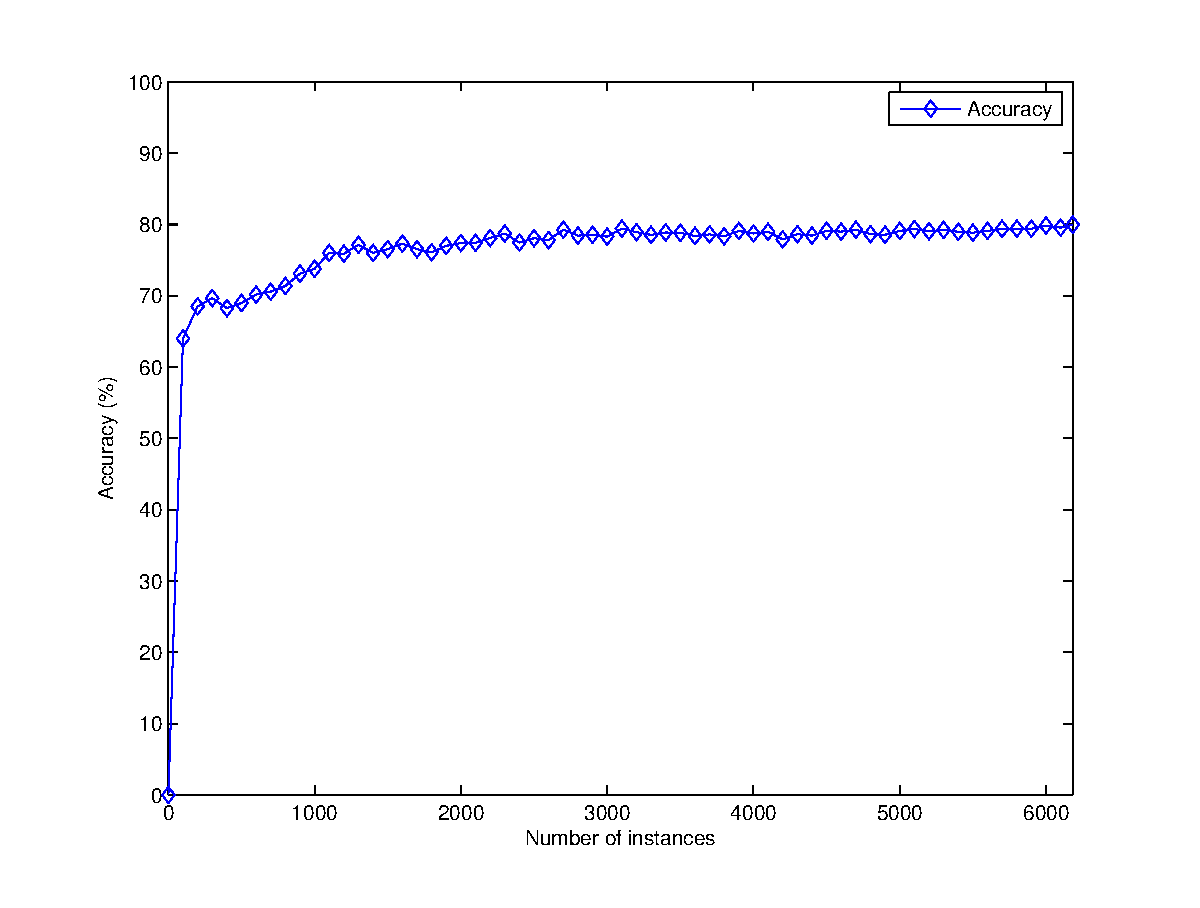
\includegraphics[scale=0.5]{bagging_accuracy.eps}
    \caption{Accuracy of linear kernel SVM based bagging ensemble as measured against the number of instances}
    \label{bagging_accuracy}
\end{figure}

On the other hand, Figure~\ref{bagging_n_models} suggests that the accuracy of a bagging based ensemble does not vary a lot with the total number of models being used underneath. A maximum accuracy of 81.33\% is observed for 7 classifiers, while the minimum value is 72.43\% for 2 classifiers.
\begin{figure}
    \centering
    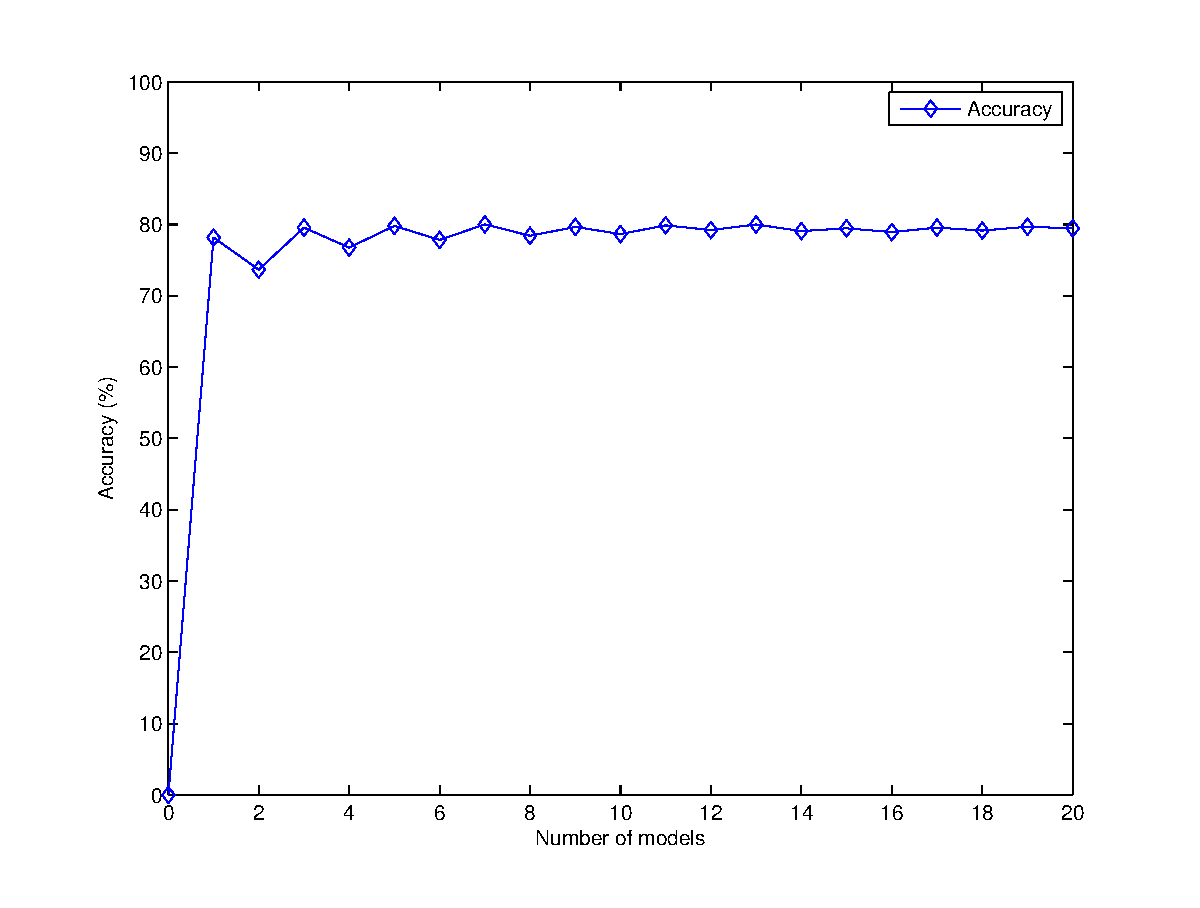
\includegraphics[scale=0.5]{bagging_n_models.eps}
    \caption{Change in accuracy of a bagging based ensemble with the number of models}
    \label{bagging_n_models}
\end{figure}

\subsubsection{Boosting}
Boosting follows a different approach to ensemble learning, by combining classifiers in a way that each successive classifier gets more incentive to classify correctly the points which the previous classifier misclassified. As shown in Figure~\ref{boosting_accuracy}, the performance of a 9-classifier ensemble peaks at 80.38\%, and does not vary a lot as the number of instances increases.
\begin{figure}
    \centering
    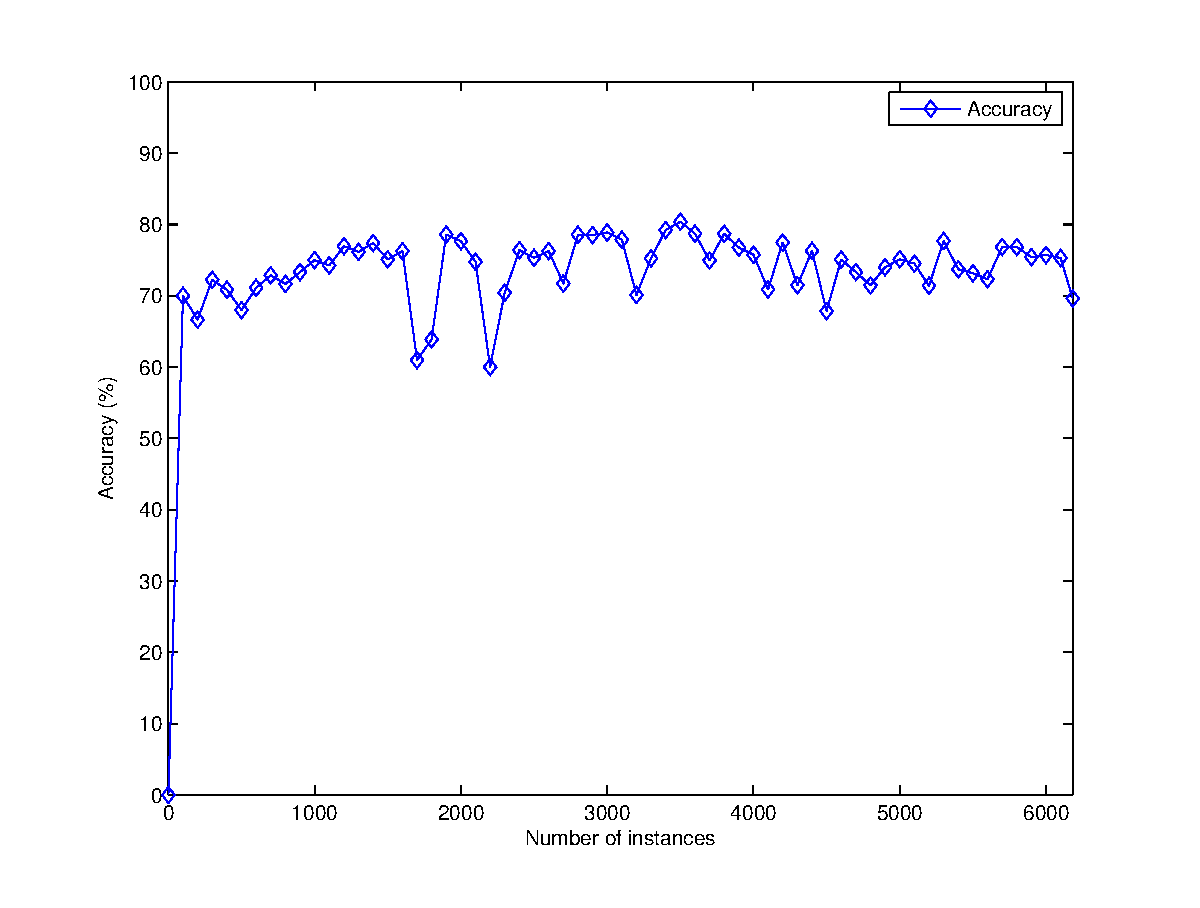
\includegraphics[scale=0.5]{boosting_accuracy.eps}
    \caption{Accuracy of linear kernel SVM based boosting ensemble as measured against the number of instances}
    \label{boosting_accuracy}
\end{figure}

\subsubsection{Stacking}
Stacking follows a more meta-level appraoch to classification, by training two levels of classifiers to perform the final classification. It can be seen in Figure~\ref{stacking_accuracy} that the performance of stacked classifiers increases with the total number of instances, similar to the other two methods of ensemble learning.
\begin{figure}
    \centering
    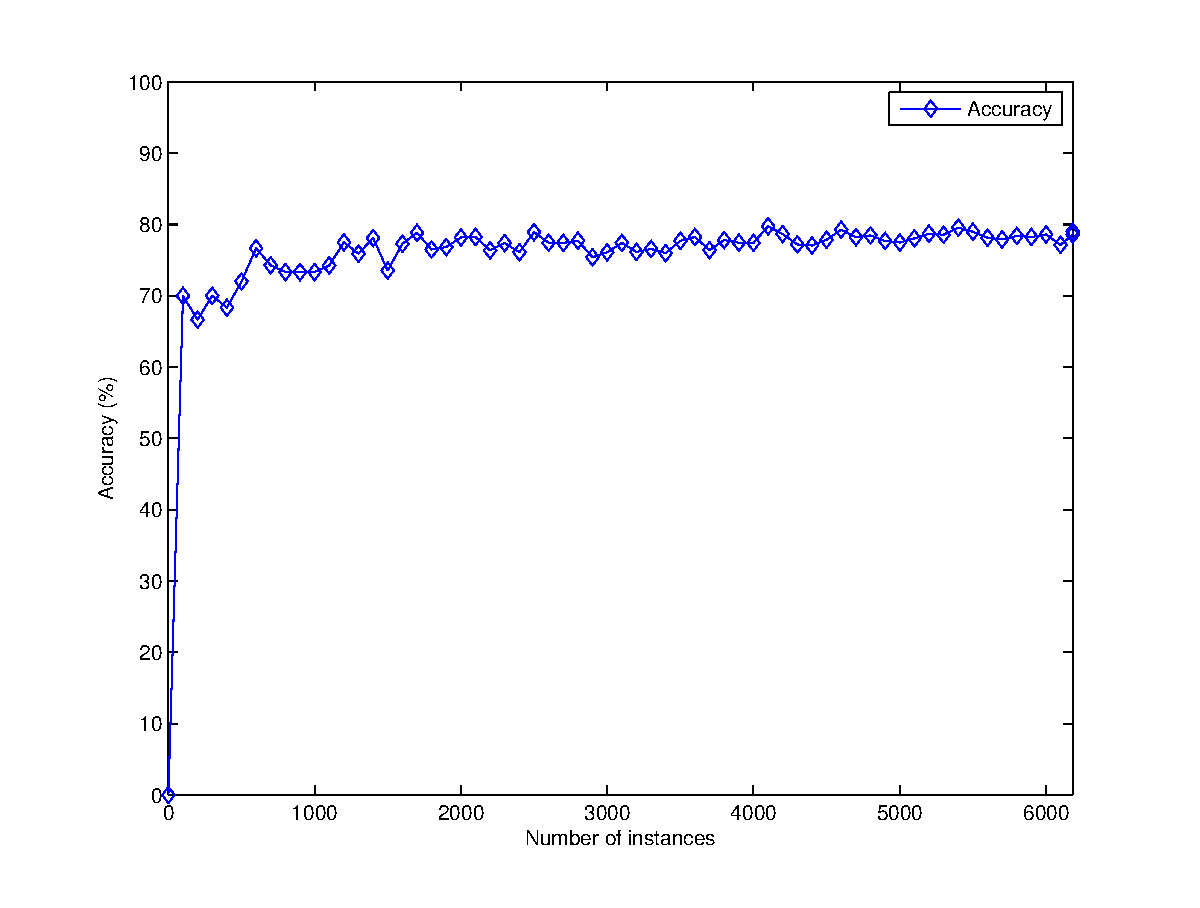
\includegraphics[scale=0.5]{stacking_accuracy.eps}
    \caption{Accuracy of linear kernel based stacking ensemble as measured against the number of instances}
    \label{stacking_accuracy}
\end{figure}

\section{System Details}
\label{section:system_details}

The second major contribution of this thesis is a web based system that allows users to perform (broadly) the following functions - help build the training data, evaluate a level of distress amongst the general public, and find out particular people who have been posting content that appears to be distressed and qualifies as needing-attention.

Specifically, users can assign labels to stories fetched from reddit, which helps in building training data while tapping into crowd intelligence. The \emph{monitoring} module then presents information about a general level of distress amongst people who are posting on Twitter (grouped by date), and about certain tweets that have been classified as depressed. Showing information about particular tweets which have been classified as depressed presents authors of the tweet which may need further attention in the form of psychological help.

The system is divided into two modules - \emph{Ratings} and \emph{Monitoring}. This choice is presented to a user as soon as they visit the front page of the web interface, as shown in Figure~\ref{landing}.
\begin{figure}
    \centering
    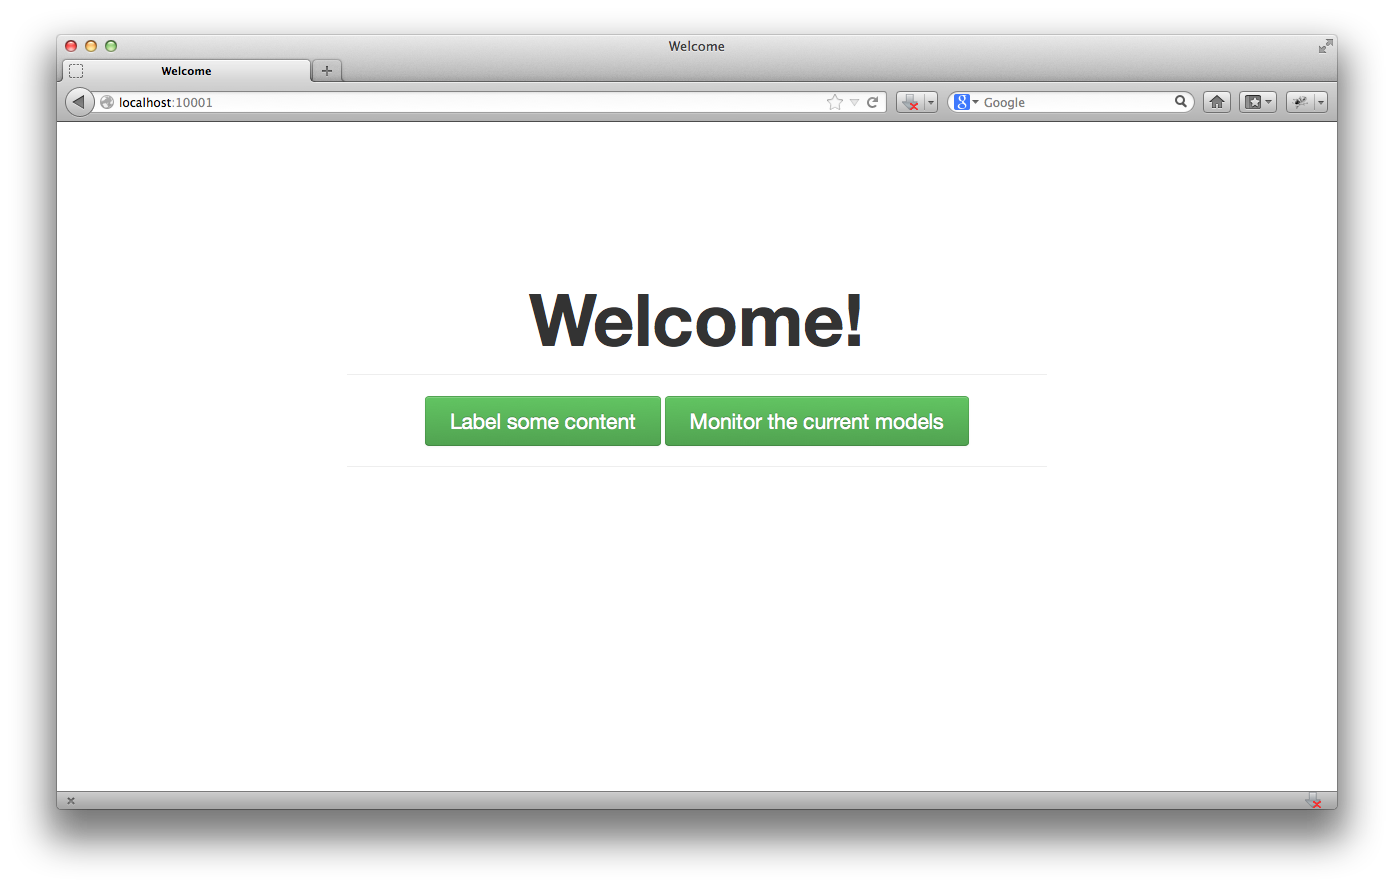
\includegraphics[width=\textwidth,scale=0.5]{landing.png}
    \caption{Landing page}
    \label{landing}
\end{figure}

The flow of the entire system can be seen as being divided into two parts. The first part, which is more manual, includes users fetching stories (from reddit) and labelling them, which helps in building the training data. The second part is built using automatic cron jobs (pieces of code that are executed after specific intervals of time), and involves the following -
\begin{itemize}
    \item{every 3 hours - fetching 100 tweets from the public stream of Twitter}
    \item{every morning - assigning labels to all tweets fetched from Twitter according to the updated model}
\end{itemize}

\section{Ratings}
The \emph{Ratings} module is built to help consolidate the training data. Users are provided with options to label the unlabeled data (as ``depressed'' or ``not depressed'') that is already present in the database. If in case there are no unlabeled stories left, then there also exists an option to fetch more data from Reddit. When invoked, this option fetches 500 stories each from \href{http://www.reddit.com/r/happy}{/r/happy} and \href{http://www.reddit.com/r/suicidewatch}{/r/suicidewatch}.

As shown in Figure~\ref{ratings}, the user is presented with a random piece of text that was fetched from Reddit, and two buttons for assigning this story a label.

\begin{figure}
    \centering
    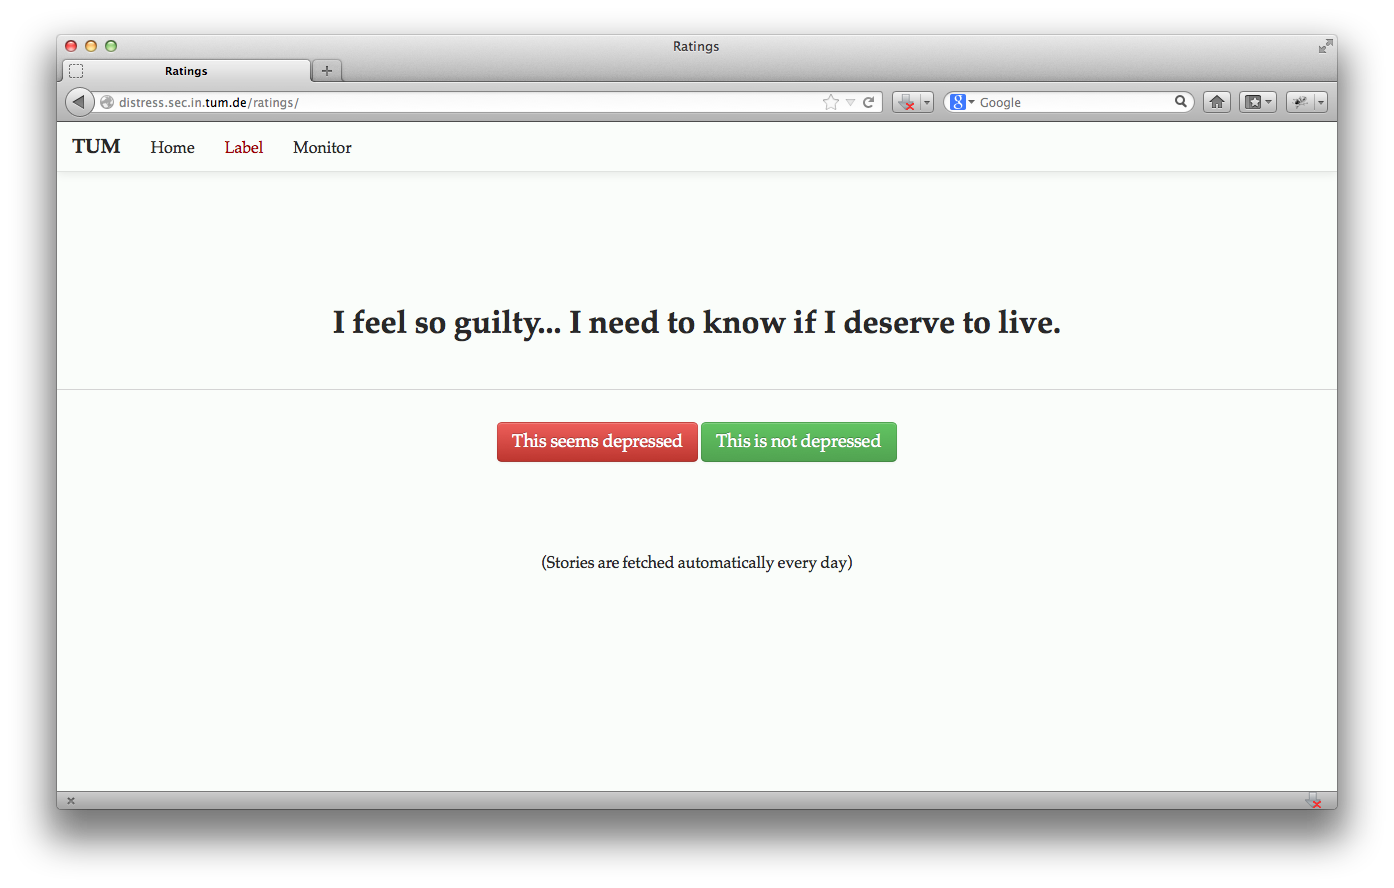
\includegraphics[width=\textwidth,scale=0.5]{ratings.png}
    \caption{Ratings module}
    \label{ratings}
\end{figure}

\section{Monitoring}
